\documentclass{article}
\usepackage{graphicx}
\usepackage{amsmath}
\usepackage{tikz}
\usepackage{float}
\usepackage[paper=letterpaper,left=25mm,right=25mm,top=3cm,bottom=25mm]{geometry}

\newtheorem{theorem}{Theorem}
\newtheorem{lemma}{Lemma}
\newtheorem{corollary}{Corollary}


\title{First Read of Your Paper}
\author{Matt Bull-Weizel, Emily Chu, Nour Hanafi, Justin Lawrence, Young Lin}
\date{52793460, 26625426, 55450928, 47260310, 54587282}

\begin{document}

\maketitle

\section{List of terms not covered in MATH 443}
% todo add defns
\begin{itemize}
\item G is a \textbf{signed graph} if every \(e \in E(G)\) is associated with a sign (+ or \(-\)). 
    \begin{itemize} 
        \item These edges are respectively called \textbf{positive edges} and \textbf{negative edges}.
        \item The \textbf{positive degree} of a vertex (denoted \(deg^+(v)\)) is the nonnegative number of positive edges incident to \(v\) in a signed graph. Similarly, the \textbf{negative degree} \(deg^-(v)\) is the nonnegative number of negative edges incident to \(v\).
    \end{itemize}
\item The \textbf{signed degree} \(sdeg(v)\) of a vertex \(v\) is \(deg^+(v) - deg^-(v)\). Note that the \textbf{degree} of a vertex in a signed graph ignores signs, so \(deg(v) = deg^+(v) + deg^-(v)\).
% polynomial-time algorithm ??? don't know if this is important to the result or not
\item A sequence of integers is \textbf{\(s\)-graphical} if it is the signed degree sequence of a signed graph.
\item A sequence of integers \(\sigma: d_1, d_2, \dots d_p\) is \textbf{standard} if  \(p-1 \ge d_1 \ge d_2 \ge \dots \ge d_p\) and \(d_1 \ge |d_p|\).
\item A \textbf{signed tree} is a signed graph that is a tree.
\item Assume \(G = (V, E)\) is a signed graph of \(p\) vertidces and \(q\) edges. Then \(q^+\) and \(q^-\) denotes the number of positive edges and negative edges of \(G\); \(p_+, p_0, p_-\) denotes the number of vertices with positive, zero and negative signed degrees.
\end{itemize}

\section{Exercises}
\begin{enumerate}
    \item Let \(S_1: 6, 2, 1, 0, 0, -1, -5, -7\) be the list of signed degrees of the vertices in a signed graph. Is \(S\) standard, and why? If not, construct a standard sequence from \(S_1\).
    
    In this case, $p = 8$ and so $p - 1 \geq 6$. However, $6 < \lvert -7 \rvert$. So, $S_1$ is not standard. Hence, we know that $-S_1: 7, 5, 1, 0, 1, -2, -6$ is standard. It's clear that $S_1$ is graphical if and only if $-S_1$ is graphical, this indicates the usefulness of standard sequences.
    
    \item Let \(S_2: 2, 2, 0, 0, 0, -2, -3 \). Construct a signed graph with \(S_2\) as its signed degree sequence.
    \begin{figure}[H]
        \centering
        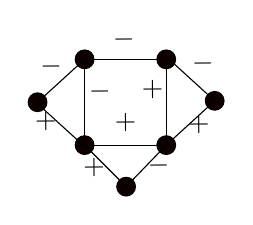
\begin{tikzpicture}[x=0.75pt,y=0.75pt,yscale=-1,xscale=1]
%uncomment if require: \path (0,300); %set diagram left start at 0, and has height of 300
    \centering
    %Shape: Circle [id:dp17545517253680176] 
    \draw  [fill={rgb, 255:red, 15; green, 0; blue, 0 }  ,fill opacity=1 ] (240.33,118.83) .. controls (240.33,116.35) and (242.35,114.33) .. (244.83,114.33) .. controls (247.32,114.33) and (249.33,116.35) .. (249.33,118.83) .. controls (249.33,121.32) and (247.32,123.33) .. (244.83,123.33) .. controls (242.35,123.33) and (240.33,121.32) .. (240.33,118.83) -- cycle ;
    %Shape: Circle [id:dp6328708315835571] 
    \draw  [fill={rgb, 255:red, 15; green, 0; blue, 0 }  ,fill opacity=1 ] (279.67,118.83) .. controls (279.67,116.35) and (281.68,114.33) .. (284.17,114.33) .. controls (286.65,114.33) and (288.67,116.35) .. (288.67,118.83) .. controls (288.67,121.32) and (286.65,123.33) .. (284.17,123.33) .. controls (281.68,123.33) and (279.67,121.32) .. (279.67,118.83) -- cycle ;
    %Shape: Circle [id:dp7265639894467566] 
    \draw  [fill={rgb, 255:red, 15; green, 0; blue, 0 }  ,fill opacity=1 ] (240.33,160.17) .. controls (240.33,157.68) and (242.35,155.67) .. (244.83,155.67) .. controls (247.32,155.67) and (249.33,157.68) .. (249.33,160.17) .. controls (249.33,162.65) and (247.32,164.67) .. (244.83,164.67) .. controls (242.35,164.67) and (240.33,162.65) .. (240.33,160.17) -- cycle ;
    %Shape: Circle [id:dp7519278663773508] 
    \draw  [fill={rgb, 255:red, 15; green, 0; blue, 0 }  ,fill opacity=1 ] (279.67,160.17) .. controls (279.67,157.68) and (281.68,155.67) .. (284.17,155.67) .. controls (286.65,155.67) and (288.67,157.68) .. (288.67,160.17) .. controls (288.67,162.65) and (286.65,164.67) .. (284.17,164.67) .. controls (281.68,164.67) and (279.67,162.65) .. (279.67,160.17) -- cycle ;
    %Shape: Circle [id:dp4345014339586212] 
    \draw  [fill={rgb, 255:red, 15; green, 0; blue, 0 }  ,fill opacity=1 ] (260.33,180.17) .. controls (260.33,177.68) and (262.35,175.67) .. (264.83,175.67) .. controls (267.32,175.67) and (269.33,177.68) .. (269.33,180.17) .. controls (269.33,182.65) and (267.32,184.67) .. (264.83,184.67) .. controls (262.35,184.67) and (260.33,182.65) .. (260.33,180.17) -- cycle ;
    %Shape: Circle [id:dp8237540788403314] 
    \draw  [fill={rgb, 255:red, 15; green, 0; blue, 0 }  ,fill opacity=1 ] (217.67,139.5) .. controls (217.67,137.01) and (219.68,135) .. (222.17,135) .. controls (224.65,135) and (226.67,137.01) .. (226.67,139.5) .. controls (226.67,141.99) and (224.65,144) .. (222.17,144) .. controls (219.68,144) and (217.67,141.99) .. (217.67,139.5) -- cycle ;
    %Shape: Circle [id:dp9976090633061713] 
    \draw  [fill={rgb, 255:red, 15; green, 0; blue, 0 }  ,fill opacity=1 ] (303,138.83) .. controls (303,136.35) and (305.01,134.33) .. (307.5,134.33) .. controls (309.99,134.33) and (312,136.35) .. (312,138.83) .. controls (312,141.32) and (309.99,143.33) .. (307.5,143.33) .. controls (305.01,143.33) and (303,141.32) .. (303,138.83) -- cycle ;
    %Straight Lines [id:da6850861947422446] 
    \draw    (244.83,118.83) -- (244.83,160.17) ;
    %Straight Lines [id:da8115526625959726] 
    \draw    (284.17,118.83) -- (284.17,160.17) ;
    %Straight Lines [id:da5923950507316124] 
    \draw    (284.17,160.17) -- (249.33,160.17) ;
    %Straight Lines [id:da5083829566701059] 
    \draw    (284.17,160.17) -- (264.83,180.17) ;
    %Straight Lines [id:da29540986015077664] 
    \draw    (264.83,180.17) -- (244.83,160.17) ;
    %Straight Lines [id:da7586058621237911] 
    \draw    (307.5,138.83) -- (284.17,160.17) ;
    %Straight Lines [id:da3978329080603926] 
    \draw    (284.83,118.17) -- (307.5,138.83) ;
    %Straight Lines [id:da5778157650059541] 
    \draw    (222.67,140.67) -- (245.33,161.33) ;
    %Straight Lines [id:da17708266002144823] 
    \draw    (244.83,118.83) -- (222.17,139.5) ;
    %Straight Lines [id:da8585901308989962] 
    \draw    (284.17,118.83) -- (244.83,118.83) ;
    
    % Text Node
    \draw (242.91,165.36) node [anchor=north west][inner sep=0.75pt]  [rotate=-359.59]  {$+$};
    % Text Node
    \draw (258.08,143.7) node [anchor=north west][inner sep=0.75pt]  [rotate=-359.59]  {$+$};
    % Text Node
    \draw (271.08,127.69) node [anchor=north west][inner sep=0.75pt]  [rotate=-359.59]  {$+$};
    % Text Node
    \draw (293.41,144.52) node [anchor=north west][inner sep=0.75pt]  [rotate=-359.59]  {$+$};
    % Text Node
    \draw (219.69,142.89) node [anchor=north west][inner sep=0.75pt]  [rotate=-359.59]  {$+$};
    % Text Node
    \draw (274.02,164.52) node [anchor=north west][inner sep=0.75pt]  [rotate=-359.59]  {$-$};
    % Text Node
    \draw (245.69,128.85) node [anchor=north west][inner sep=0.75pt]  [rotate=-359.59]  {$-$};
    % Text Node
    \draw (257.19,103.85) node [anchor=north west][inner sep=0.75pt]  [rotate=-359.59]  {$-$};
    % Text Node
    \draw (295.36,115.12) node [anchor=north west][inner sep=0.75pt]  [rotate=-359.59]  {$-$};
    % Text Node
    \draw (222.16,116.62) node [anchor=north west][inner sep=0.75pt]  [rotate=-359.59]  {$-$};
    

    \end{tikzpicture}
    \end{figure}      

\newpage
    
    \item Is \(S_3: 6, 2, 1, 0, 0, -1, -5, -7\) a signed degree sequence of a signed graph?

    To determine whether $S_3$ is a degree sequence, we must consider $-S_3$ since $S_3$ is not standard s shown in 1. So we let $S = -S_3: 7, 5, 1, 0, 0, -1, -2, -6$. We see that $d_{d_1 + 1} = -6$ so $m$ is forced to be $0$ in theorem 3. We apply it the operation in theorem 3 getting
        \begin{align*}
            & 7, 5, 1, 0, 0, -1, -2, -6 \\
            & 4, 0, -1, -1, -2, -3, -7
        \end{align*}
    The sequence $Q: 4, 0, -1, -1, -2, -3, -7$ is not standard, additionally, $-Q$ is not standard since the size of the sequence is $7$ but $d_1$ is $7$. So, $Q$ cannot be graphical, meaning that $-S_3$ cannot be graphical and in particular, $S_3$ is not graphical.
\end{enumerate}

\section{Main result(s) of the paper}

This paper gives necessary and sufficient conditions for an integral sequence
to be the signed degree sequence of a signed graph or a signed tree, answering a
question raised by Chartrand et al. (1994). 

\addtocounter{theorem}{2}

\begin{theorem}
    A standard integral degree sequence 
    \begin{equation}
        \sigma: d_1,d_2,d_3,\ldots, d_p
    \end{equation}
is graphical if and only of 
\begin{equation*}
    \sigma_m':d_2-1,\ldots d_{d_1+m+1}-1,d_{d_1+m+2},\ldots, d_{p-m},d_{p-m+1}+1,\ldots,d_p+1
\end{equation*}
 is \textbf{s-graphical}, where $m$ is the maximum non-negative integer such that $d_{d_1+m+1}>d_{p-m+1}.$
\end{theorem}

\addtocounter{theorem}{3}

\begin{theorem}
    Suppose $\sigma : d_1,...,d_p$ is an integral sequence of $p \geq 2$ terms. Suppose $\sigma$ has $p_+$ positive terms, $p_0$ zero terms and $p_-$ negative terms. Let $\delta = 1$ if $p_+p_- > 0$ and $\delta = 0$ otherwise. Then, Then $\sigma$ is the signed degree sequence of a signed tree if and only if (T1) to (T4) hold.
        \begin{itemize}
            \item[(T1)] $\sum_{i = 1}^{p} d_i \equiv 2p - 2 \pmod 4$
            \item[(T2)] $\sum_{i = 1}^{p} \lvert d_i \rvert \le 2p - 2 - 2p_0$
            \item[(T3)] $\sum_{i = 1}^{p} \lvert d_i \rvert + 2\sum_{d_i < 0} \lvert d_i \rvert \leq 2p - 2 - 4\delta + 4p_-$
            \item[(T4)] $\sum_{i = 1}^{p} \lvert d_i \rvert + 2\sum_{d_i > 0} \lvert d_i \rvert \leq 2p - 2 - 4\delta + 4p_+$
        \end{itemize}
\end{theorem}

\newpage

\section{Other results used in the paper}

\begin{lemma}
    If \(\sigma: d_1, d_2,\cdots,d_p\) is the signed degree sequence of a signed graph \(G\), then \(-\sigma: -d_1, -d_2,\cdots,-d_p\) is the signed degree sequence of the signed graph \(G'\) obtained from \(G\) by interchanging positive edges with negative edges.
\end{lemma}

\addtocounter{theorem}{-6}

\begin{theorem}
    \textbf{[Chartrand et al.]} A standard integral degree sequence 
    \begin{equation*}
        \sigma: d_1,d_2,d_3,\ldots, d_p
    \end{equation*}
    is graphical if and only of 
    \begin{equation*}
        \sigma':d_2-1,\ldots d_{d_1+s+1}-1,d_{d_1+s+2},\ldots, d_{p-s},d_{p-s+1}+1,\ldots,d_p+1
    \end{equation*}
    is \textbf{s-graphical} for some $s$, where $0 \leq s \leq (p - 1 - d_1)/2$.
\end{theorem}

\addtocounter{lemma}{2}

\begin{lemma}    \textbf{[Chartrand et al.]} If \(G = (V, E)\) is a signed graph, then \(k=\sum_{v\in V} sdeg(v)\equiv 2q \pmod{4}, q^+ = \frac{1}{4} (2q+k)\) and \(q^- = \frac{1}{4} (2q-k)\)
\end{lemma}

\addtocounter{corollary}{7}

\begin{corollary}
    Suppose \(\sigma: d_1, d_2, \cdots, d_p\) is an integral sequence of \(p\ge 3\) terms. Suppose \(\sigma\) has at least two terms in which \(|d_i| = 1, d_p = 1\), and one of the following conditions holds:
    \begin{enumerate}
        \item \(|d_i| \le 1\) for \(1\le i\le p, d_1\ge 0\) and \(d_1 = 0\) if \(p_0 > 0\).
        \item \(d_1 \ge 2\)
        \item \(d_i\le 1\) but \(d_i \ne -1\) for \(1\le i\le p\) and \(d_1 = 0\) and \(\delta =1\).
        \item \(d_i = 1\) or \(d_i\le -2\) for \(1\le i\le p\) and \(d_1 = \delta = 1\)
    \end{enumerate}
    Then \(\sigma\) is the signed degree sequence of a signed tree if and only if \(\sigma': d_1 -1 , d_2, \cdots,d_{p-1}\) is the signed degree sequence of a signed tree.
\end{corollary}

\section{Future directions}

Given a fixed partially ordered Abelian group $(K, +, \geq)$ we can define a $K$-graph $G$ as a (finite) graph $(V,E)$ where each $e \in E$ is given an associated element of $K$ (call it $e_K$). Let $E(v) = \{ xy \in E : x = v \}$ be the set of edges incident to $v$. We may then define the $K$-degree as $K\text{-}\deg(v) = \sum_{e \in E(v)} e_K$. 

Hence, given a sequence $d_1 \geq d_2 \geq ... \geq d_n$ in an Abelian group $K$, when can we find a $K$-graph $G$ with vertex set $\{ v_1, ..., v_n \}$ such that $K\text{-}\deg(v_i) = d_i$? 




\nocite{*}
\bibliographystyle{plain}
\bibliography{citations}

\end{document}
